
\section{Motivation}
% Why is SLR important?
% How much will SL rise?
% Largest uncertainty from Antarctica

Improving projections of the rate of global sea level rise in response to a warming world is vital for effectively mitigating future environment and socio-economic impacts \citep{durandsealevel2022}. A large portion of the uncertainties in modern and projected sea level rise is related to the contribution from the Antarctic Ice Sheet \citep[Figure \ref{fig:chp1_SLR}b, ][]{bamberice2022, edwardsprojected2021, slaterantarctic2018, otosakamass2023}. The Antarctic Ice Sheet contains a total volume of ice equivalent to 57.2 m of sea level rise \citep{fretwellbedmap22013}. Satellite observations show that Antarctica contributed $\sim7.4$ mm to mean sea level since 1992 \citep{otosakamass2023}, and of the various components of sea level rise, the contribution from Antarctica is accelerating the fastest \citep[Figure \ref{fig:chp1_SLR}a, ][]{neremclimatechangedriven2018}. Since the early 1990s, the sea level contribution from Antarctica has increased by 25\% \citep{otosakamass2023}. By the end of the century, Antarctica is projected to contribute between 0.03 and 0.28 m to mean sea level \citep[RCP 8.5,][]{intergovernmentalpanelonclimatechangeipccocean2022}. Optimal strategies for preparing coastal communities to best mitigate the impacts of rising sea level depends on where in this range of uncertainties the true sea level rise will be. Some of the uncertainty in how the Antarctic Ice Sheet will respond to a warming world stems from a lack of understanding of the complex interactions between the ice and the underlying earth \citep[e.g.][]{schlegelexploration2018, zhaobasal2018}.

% \begin{figure}[!ht]
%     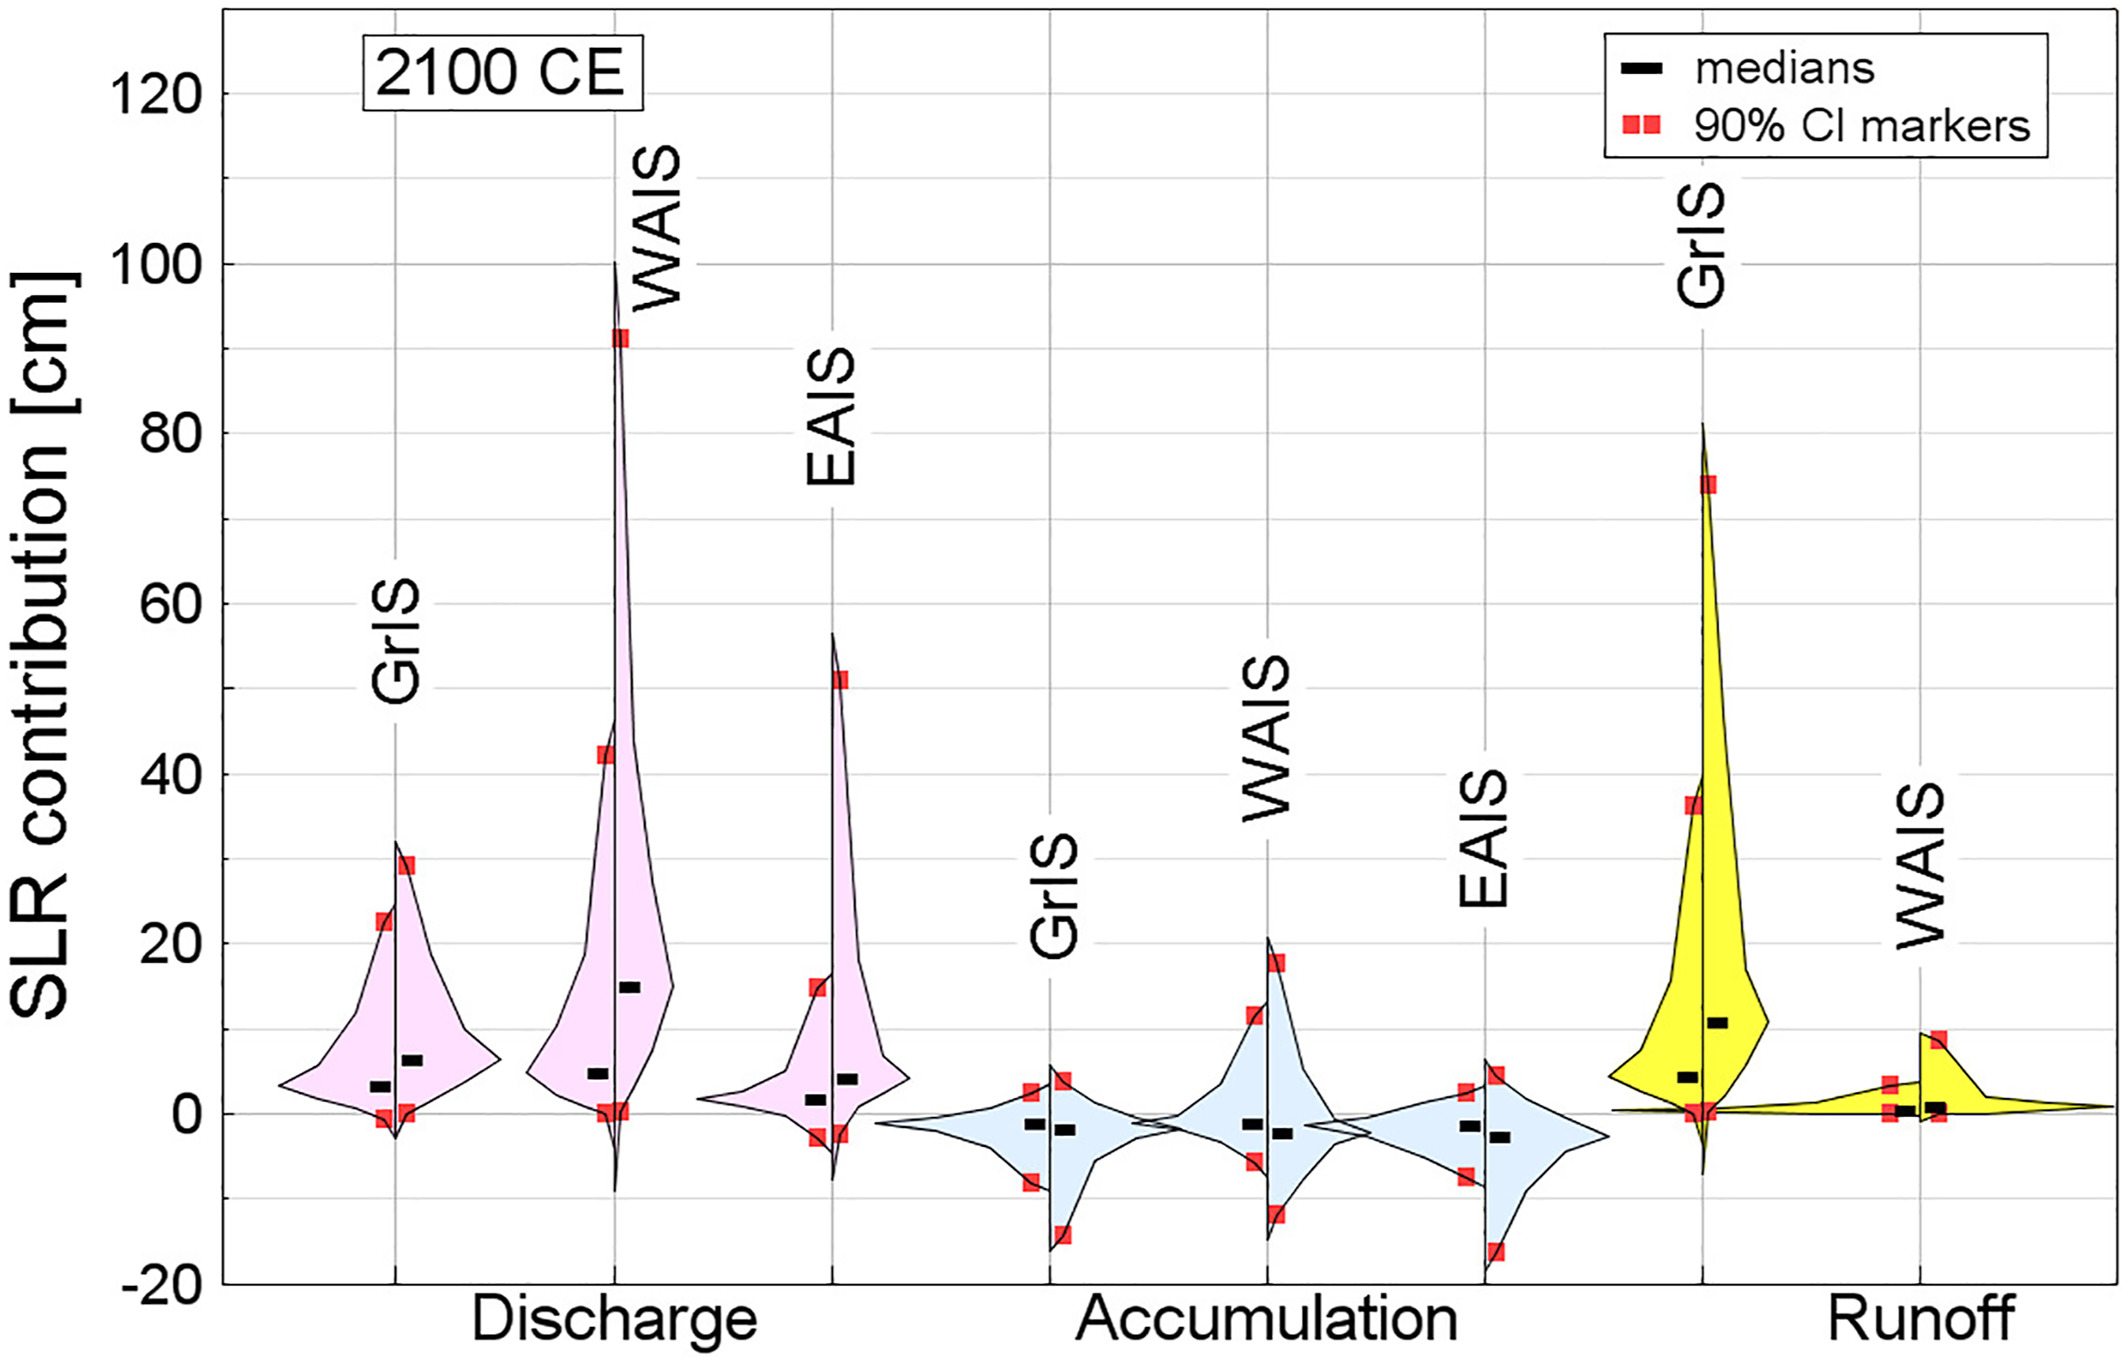
\includegraphics[width=.6\textwidth]{figures/chp1/bamber2022_SLR_uncertainty.jpg}
%     \caption{Probability distributions for projected global sea level rise contributions for the year 2100 from the Greenland Ice Sheet (GrIS), West Antarctic Ice Sheet (WAIS), and East Antarctic Ice Sheet (EAIS), separated into three processes; discharge, accumulation, and runoff. Left and right sides of each distribution show the +2$^{\circ}$C and +5$^{\circ}$C global temperature trajectories, respectively. Figure from \citet{bamberice2022}.}
%     \label{fig:chp1_SLR}
% \end{figure}

\begin{figure}[!ht]
  \centering
    \begin{subfigure}[t]{.54\textwidth}
        \centering
        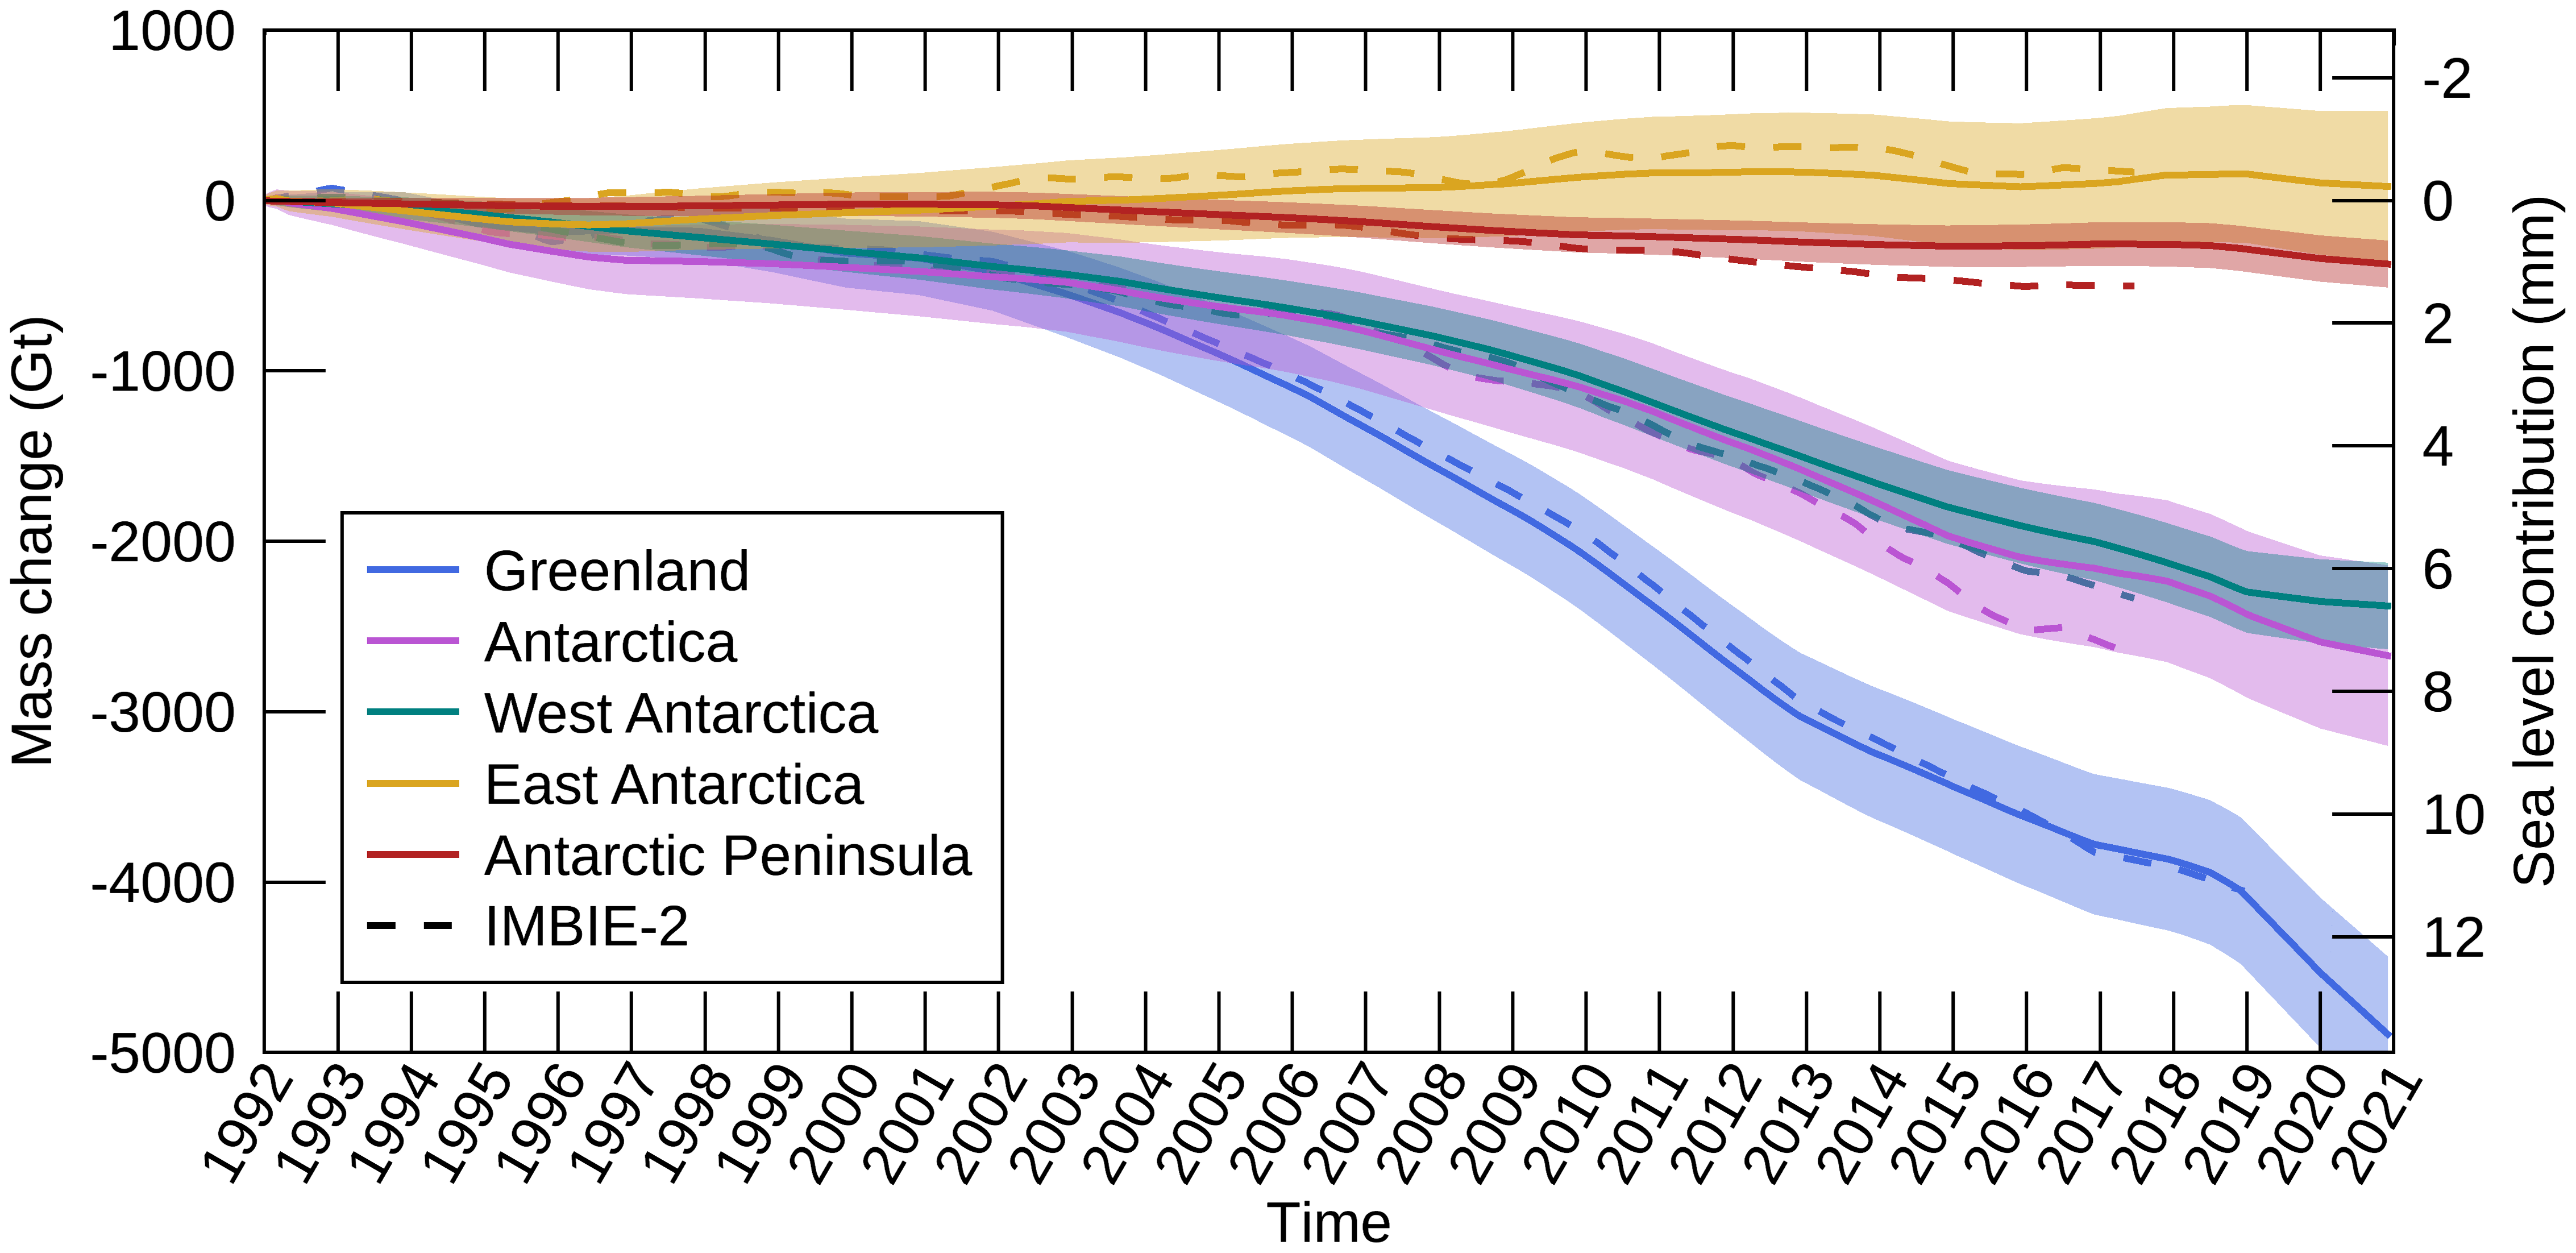
\includegraphics[width=\textwidth]{figures/chp1/Otosaka2023_mass_change.png}
        \caption{}
    \end{subfigure}
    \begin{subfigure}[t]{.44\textwidth}
        \centering
        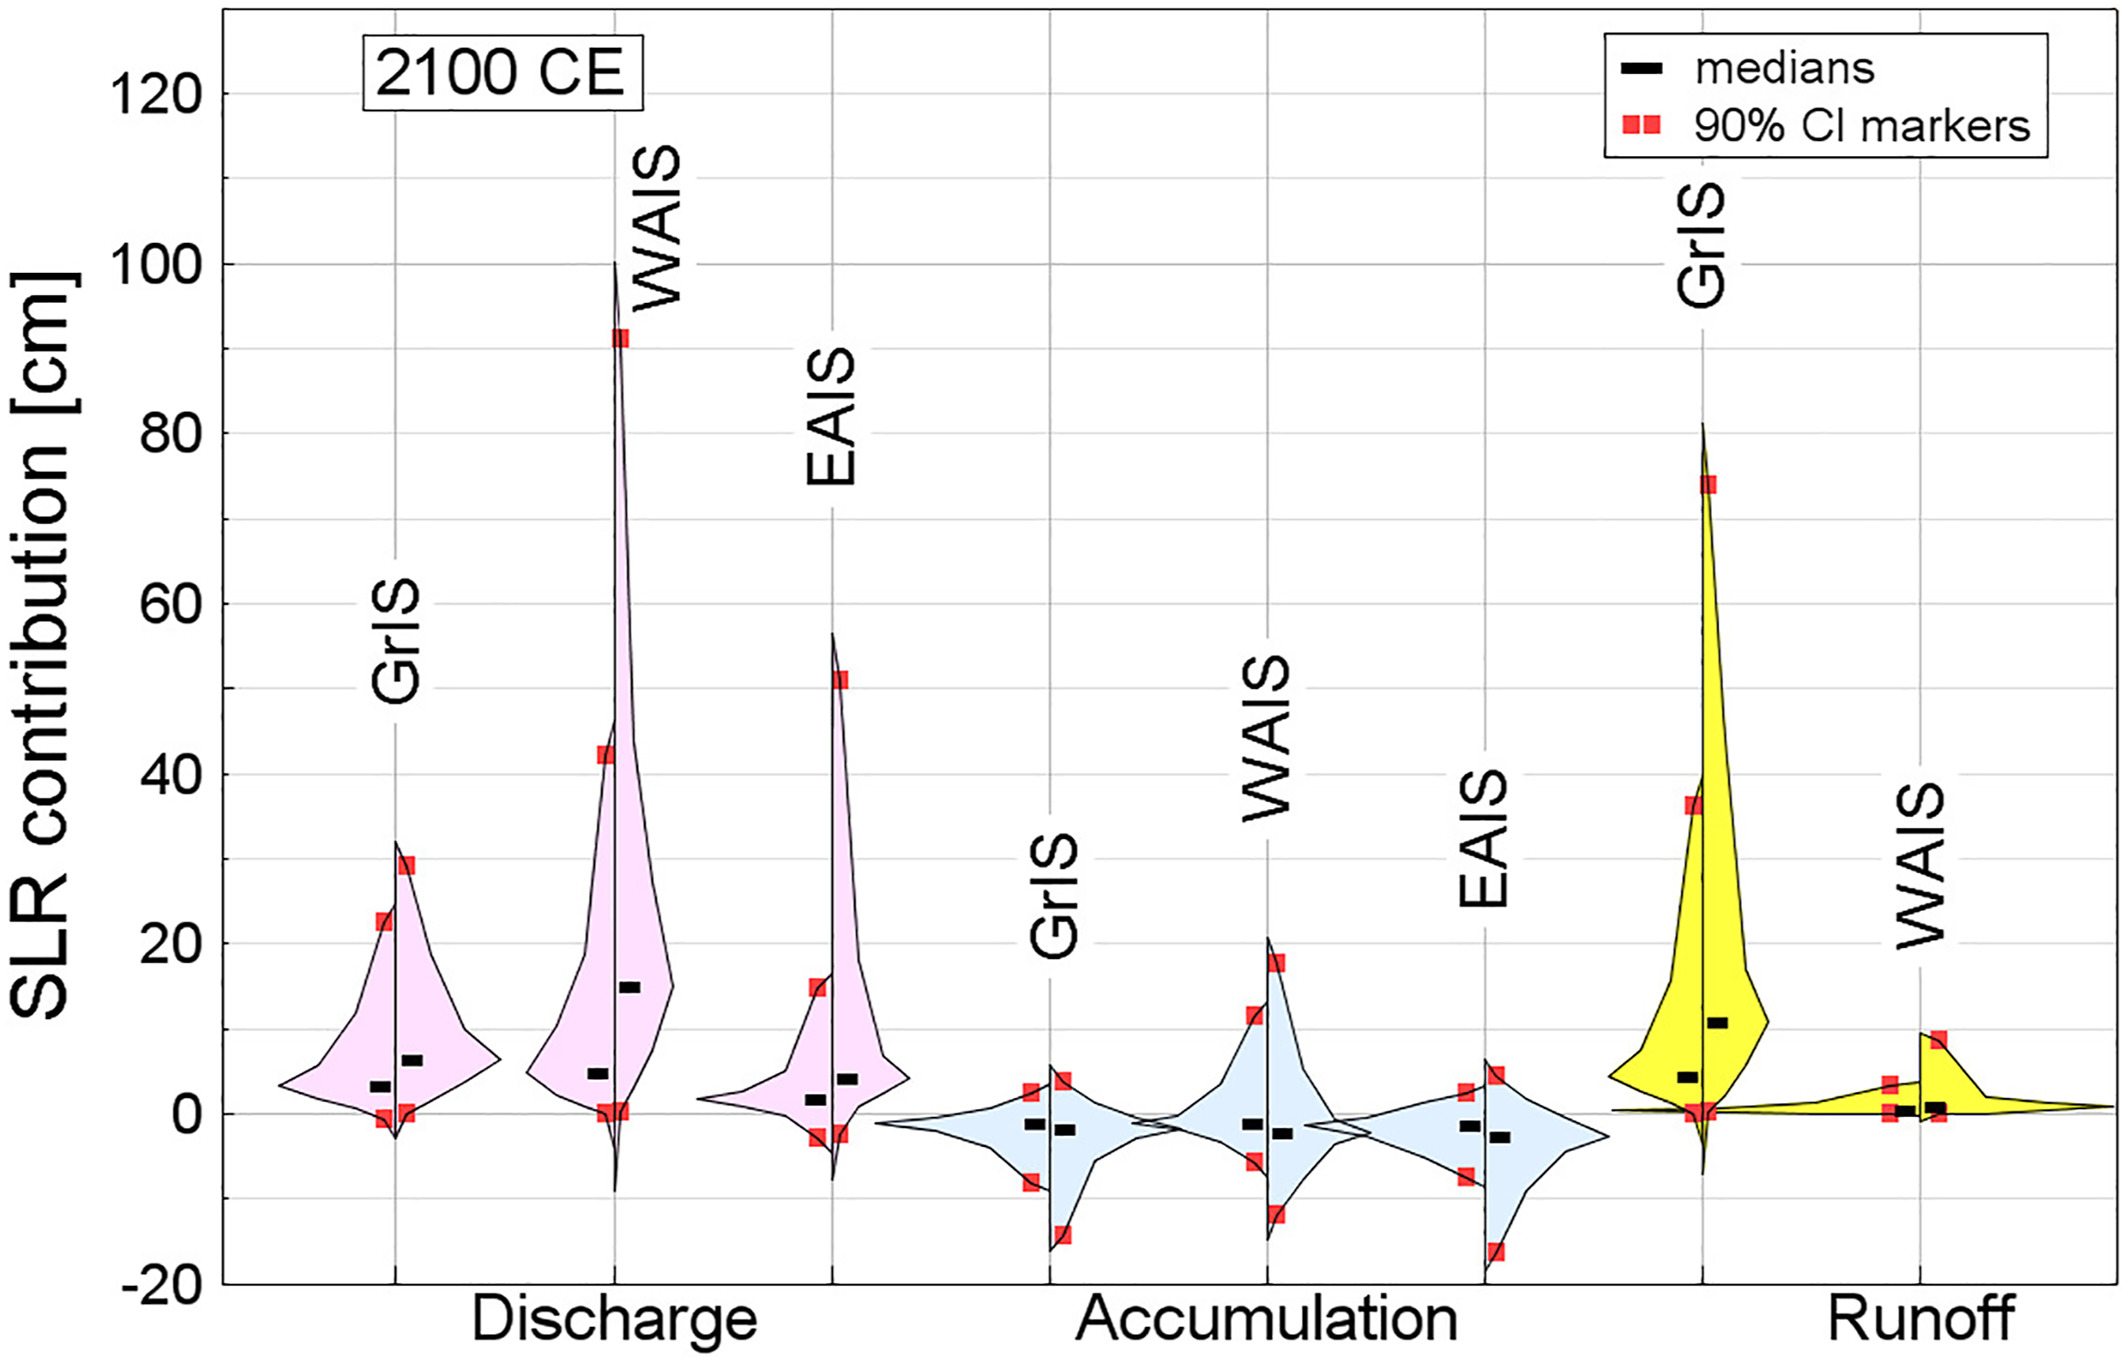
\includegraphics[width=\textwidth]{figures/chp1/bamber2022_SLR_uncertainty.jpg}
        \caption{}
    \end{subfigure}
  \caption[Past observations and future predictions of sea level rise]{Past observations and future predictions of sea level rise.
  \textbf{a)} Observed cumulative mass change and sea level contributions from the various ice sheets. Data comes from satellite-altimetry estimates of volume changes, gravimetric estimates of mass changes, and quantification of input-output fluxes. Figure from \citet{otosakamass2023}.
  \textbf{b)} Probability distributions for projected global sea level rise contributions for the year 2100 from the Greenland Ice Sheet (GrIS), West Antarctic Ice Sheet (WAIS), and East Antarctic Ice Sheet (EAIS), separated into three processes; discharge, accumulation, and runoff. Left and right sides of each distribution show the +2$^{\circ}$C and +5$^{\circ}$C global temperature trajectories, respectively. Figure from \citet{bamberice2022}.}
    \label{fig:chp1_SLR}
\end{figure}

\section[Influences on ice dynamics]{Influence of bathymetry, topography, and geology on ice dynamics\sectionmark{Influences on ice dynamics}}
% \section{Influences on ice dynamics}

The underlying Earth influences ice sheets through several mechanisms, which I group as those resulting from bedrock topography, geologic structures, and bedrock physical properties. Here I describe each of these categories of influences on the Antarctic Ice Sheet, followed by introducing the specific study area, the Ross Ice Shelf.   

\subsection{Bedrock topography}
% confinement / slope controls speed ()
% physiographic steering of ice / water (Holland model 2018, Tinto et al. 2019, halberstadticesheet2016, andersonseismic2019)
% control on erosion / deposition (lee/stoss sides of ridges) (Cuffey and Paterson 2010)
% buttressing of ice shelves ()
% GIA feedbacks (couloncontrasting2021, barlettaobserved2018, kachuckrapid2020)

% we need bathymetry
% how to get bathy (airborne / over-snow radar / over-snow seismics / shipborne seismics)

Offshore bathymetry and onshore bed topography exert several fundamental controls on how the Antarctic Ice Sheet behaves. Offshore, where the ice is floating, the influence of the bathymetry is limited to the guiding of ocean circulations. Bathymetric ridges have been shown to block, or re-direct, the inflow of melt-inducing waters to the ocean cavity beneath floating ice shelves \citep{derydtgeometric2014, zhaosillinfluenced2019, goldbergbathymetric2020}. Approximately 75\% of Antarctica's coastline is composed of these floating ice shelves, and 83\% of total ice discharged into the Southern Ocean from Antarctica is through these shelves, highlighting their significance to Antarctica's ice budget \citep{rignoticeshelf2013}. Of the 83\% of total ice loss from Antarctica through ice shelves, basal melt is responsible for approximately half \citep{greeneantarctic2022, rignoticeshelf2013}. Some of this melt occurs from surface waters, where bathymetry has little effect, but for many of the largest ice shelves, the majority of basal melt occurs along the deep grounding zone \citep{adusumilliinterannual2020}. Here, the melt-inducing water bodies are dense and flow into the ice shelf cavities along the seafloor \citep{hollandmodel2008, tintobathymetry2015}. Therefore, bathymetric features act to guide or block these circulations from reaching the grounding zone where they can melt the ice base. In addition to steering ocean currents, bed topography, in regions of grounded ice, acts to steer the ice flow. \\

As revealed by extensive seismic and swath bathymetry data in Antarctica's Ross Sea (Figure \ref{fig:chp1_data_coverage}a), the dynamics of an advancing or retreating ice sheet are predominantly controlled by the physiography of the bed \citep{halberstadticesheet2016, andersonseismic2019}. If large troughs and banks exist, advancing ice is initially confined by these features, while the banks remain ice-free \citep{andersonross2014}. Eventually, after the ice has covered the entire region, the retreat is initially confined to these narrow troughs, while the banks retain grounded ice for much longer \citep{andersonseismic2019, halberstadticesheet2016}. As the ice thins or retreats into regions of deeper bed topography, these banks remain grounded, while the rest of the ice sheet decouples from the bed, begins floating and forms an ice shelf \citep{shipplate1999}. This remaining grounded ice on bathymetric highs forms pinning points. \\

\begin{figure}[!ht]
    \centering
    \includesvg[inkscapelatex=false,width=0.98\textwidth]{chp1/data_coverage}
    \caption[Summary of existing geologic and geophysical data for Antarctica]{Summary of existing geologic and geophysical data for Antarctica. \textbf{a)} Map of data coverage in Antarctica indicating outcropping regions, drill core sites, seismic and  magnetotelluric surveys, and bed elevation data points of Bedmap3, mostly from airborne radio-echo sounding \citep{frémandantarctic2022}. \textbf{b)} Various methods of acquiring information sub-surface geology. Figure adapted from \citet{aitkenantarctica2023}.}
    \label{fig:chp1_data_coverage}
\end{figure}

Pinning points are regions of locally grounded ice within a floating ice shelf \citep{matsuokaantarctic2015}. The friction between the bed and ice base at these points impart a critical resisting force to the discharge of upstream ice; an effect known as buttressing \citep{thomasice1979, dupontassessment2005}. Since the base of ice shelves is flat relative to the underlying bathymetry, the morphology of the seafloor is the dominant control of the location and geometry of these pinning points. The bedrock topography has been thought to be relatively constant over a millennial timescale, meaning that pinning points' geometries vary mostly by temporal changes in the ice thickness. However, recent studies of glacial isostatic adjustment, the vertical rebound of the Earth following deglaciation, throughout West Antarctica have demonstrated high spatial variability and short (multi-centennial-to-millennial) timescales for these vertical land movements \citep{couloncontrasting2021, barlettaobserved2018, kachuckrapid2020}. As the bedrock beneath portions of West Antarctica continues to rebound, the number and extent of these pinning points will likely increase, possibly providing a stabilizing effect to the ice sheet. \\

All of these above controls on ice dynamics imparted by the physiography of the bed rely on accurate knowledge of bed topography and bathymetry. Due to the inherently challenging nature of Antarctic fieldwork, and the logistical challenge of measuring bed elevations beneath thick ice, 50\% of the Antarctic Ice Sheet is more than 5 km from the nearest measurement of bed elevation \citep[Figure \ref{fig:chp1_data_coverage}a,][]{morlighemdeep2020}. This value increases greatly if the floating ice shelves are included. For grounded ice, the dominant techniques for direct measurements of bed elevation data are airborne radio-echo sounding, over-snow radar, and seismic surveying \citep[Figure \ref{fig:chp1_data_coverage}b,][]{fretwellbedmap22013}. In the open ocean, bathymetry data are typically collected with ship-borne multibeam echo sounding, seismic surveying (Figure \ref{fig:chp1_data_coverage}b), or from satellite-altimetry. Acquiring bathymetry data beneath floating ice shelves presents a particular challenge. The efficient shipborne methods are unavailable since the ice shelves are persistent year-round, unlike the sea ice in the open ocean. Radio-echo sounding, either ground-based or airborne, cannot image through the water column. Direct observations through drilling are possible and exist, but typically require drilling through 100's to 1000's of meters of ice \citep[Figure \ref{fig:chp1_data_coverage},][]{cloughross1979, pattersonsensitivity2022}. Autonomous underwater vehicles (Figure \ref{fig:chp1_data_coverage}b) present another option, but are expensive and have limited range \citep{dowdeswellautonomous2008, nichollsmeasurements2006}. The only feasible method of direct observations of sub-ice shelf bathymetry is over-snow seismic surveying (Figure \ref{fig:chp1_data_coverage}b). However, for the vast area of many ice shelves, even sparse coverage ($\sim50$ km spacing) of seismic points across the ice shelf takes several field seasons of data acquisition \citep{bentleyross1984}. 


\subsection{Geologic structures}
% GHF (larourice2012, pollardsensitivity2005, seroussiinfluence2017)
% GHF, localization from faults (goochpotential2016, begemanspatially2017)
% radiogenic heat from crust (burton-johnsongeothermal2020)
% storage / transport of groundwater (christoffersensignificant2014)
% confinement of water -> increased pore pressure (tulaczykbasal2000, bellwidespread2011)
% enhanced GIA within fault-bound basins (peltierglacial2022, steffenglacially2021)

% we need faults, basement margins, aquifer locations
% how to get this (gravity, magnetics, magnetotellurics)
Additional influences on the overriding ice include the delivery of geothermal heat and subglacial water to the ice base and the vertical deformation of the bedrock in response to changing ice loads. Geothermal heat influences ice dynamics through several mechanisms; 1) increasing the temperature of the ice which lowers its viscosity, leading to  enhanced flow via internal deformation \citep{llubesrelations2006}, 2) meltwater lubrication of the bed reduces friction, enhancing flow \citep{pollardsensitivity2005}, and 3) increasing the ability of the bed to deform via increased pore-fluid pressure, which increases ice flow \citep{tulaczykbasal2000}. The latter two effects, while enhanced by geothermal heat through the melting of ice, also occur with simply the presence of liquid water at the ice-bed interface. As briefly mentioned in the above section, glacial isostatic adjustments of the bedrock following changes in ice load can influence the ice by altering the geometry and locations of grounded ice. \\

Each of these effects; geothermal heat flow, subglacial water availability, and glacial isostatic adjustment, are in turn influenced by geologic structures within the upper crust. A portion of subglacial water comes from either transport along the ice-bed interface, or from the melting of the ice base. However, an often overlooked component of the subglacial hydrologic system is groundwater stored in deep sedimentary aquifers. For example, hydrologic modelling of the ice streams of the Siple Coast (Figure \ref{fig:chp1_data_coverage}a) estimated the components of the hydrologic budget to be 8\% from local basal melting, 47\% from inflow from the ice sheet interior, and 45\% from groundwater reservoirs \citep{christoffersensignificant2014}. These modelling observations of extensive groundwater have been recently verified beneath the Whillans Ice Stream by a magnetotelluric survey. This survey imaged an extensive groundwater aquifer within a sedimentary basin, containing at least an order of magnitude more water than the shallow hydrologic system \citep{gustafsondynamic2022}. The vertical flow of this basinal groundwater is controlled by the pressure of the overriding ice sheet. As this overburden pressure decreases with thinning ice, groundwater is discharged to the ice base \citep{goochpotential2016, lisedimentary2022}. This discharge is likely concentrated along pre-existing weaknesses or impermeable surfaces, such as fault damage zones, or the margins of crystalline basement \citep{joliegeological2021}. During this ice-induced hydraulic unloading, regional geothermal heat is advected along the fluid pathways, leading to potentially highly elevated heat flow delivered to the ice base \citep{ravierglaciohydrogeology2018, lisedimentary2022}. In addition to concentrating both subglacial water and geothermal heat, these faults, or more generically, regions of the crust which have experienced recent faulting, will respond differently to stresses induced by glacial isostatic adjustment. To a first order, the isostatic response of the solid-earth to changing ice load is controlled by the rheology of the mantle \citep{whitehousesolid2019}. However, on a more local scale, pre-existing faults are shown to accommodate glacial isostatic rebound-induced stresses \citep{peltierglacial2022, steffenglacially2021}. \\

To be able to understand the above influences on the ice, we must have some fundamental knowledge of the geologic structures beneath the ice. This includes knowing where sedimentary basins, and possible aquifers within, are located, where faults likely intersect the ice base, and the geometry of the crystalline basement. Each of these components is difficult to image directly. Drilling, seismic surveys, or geologic analysis of rock outcrops all provide valuable information but are not feasible to cover wide regions (Figure \ref{fig:chp1_data_coverage}). Indirect methods are therefore needed. These include techniques such as gravity, magnetic, or electromagnetic methods. Each of these techniques records measurements of the spatial variation of a potential field, such as the Earth's gravity, magnetic, or electromagnetic fields. These fields are all partially dependant on a physical Earth property, such as rock density, magnetic susceptibility, or resistivity. From these relationships, sub-surface geologic information can be modelled. 


\subsection{Basal roughness}
% onset of ice streams (bellinfluence1998, anandakrishnaninfluence1998)
% effective resistance of pinning points (Still mechanical 2019)
% ice streaming (alleydeformation1986, )
% erodibility/deformation of till (alleydeformation1986)

% we need sediment thickness

The last major influence on the ice from the underlying Earth I present is the roughness of the bed which the ice sheet flows over. This bed roughness is important on both a micro and macro scale. At a micro-scale, roughness is determined by the material of which the bed is composed. A bed of erosion-resistance crystalline basement, for example, can greatly hinder the flow of ice. This material results in high friction with the ice base, slowing the sliding of ice \citep{bellinfluence1998}. Conversely, beds composed of fine-grained tills allow fast ice flow. This fast flow is predominantly due to deformation within the till as the ice flows \citep{alleydeformation1986}. In between the end members of crystalline basement and fine grain till are lithified sedimentary rocks, for example. This type of bed may initially lead to high friction with the ice, but due to their high erodability, sedimentary rock will quickly generate till \citep{anandakrishnaninfluence1998}. A macro-scale view of basal roughness is also important for ice dynamics. As observed at the Siple Coast (Figure \ref{fig:chp1_data_coverage}a) ice streams, there is a strong inverse relation between bed roughness, from scales of 5 to >40 km, and ice stream velocities \citep{siegertmacroscale2004}. The composition of the bed also plays an important role in the total effective resistance imparted on ice flow from pinning points \citep{stillmechanical2019}. \\

To best quantify the effect of basal roughness on ice dynamics, information on the material properties of the bed is needed. While sediment samples beneath the ice yield valuable information, they may only represent the bed at the specific location where they were sampled. The most fundamental information needed is the generic rock type of the bed, namely, is the bed loose, unconsolidated sediment, lithified sedimentary rock, or crystalline rock? \citet{aitkenantarctica2023} provide a detailed review of Antarctica's sedimentary basins, and the methods employed to determine both the presence of sediment and the sediment thickness. These methods, as well as the methods described in the above sections, are shown in Figure \ref{fig:chp1_data_coverage}, as reproduced from \citet{aitkenantarctica2023}. 

With the dominant influences from the underlying Earth on ice dynamics laid out, I will now introduce the study area of this thesis, Antarctica's Ross Ice Shelf. 


\section{Ross Ice Shelf}
% what is the RIS? 
% size, location, map
% importance for AIS and SLR
% past fast and large GL retreat

The Ross Ice Shelf is Antarctica's largest ice shelf ($\sim480,000$ km\textsuperscript{2}), Figure \ref{fig:chp1_data_coverage}). It is situated between the Transantarctic Mountains and Marie Byrd Land. It buttresses a catchment of ice that flows from both the East and West Antarctic Ice Sheets. This catchment contains 11.6 m of global sea level equivalent \citep{fretwellbedmap22013, rignotantarctic2011, tintoross2019}. Compared to many other ice shelves, the Ross Ice Shelf is currently relatively stable \citep{moholdtbasal2014, rignoticeshelf2013}. However, geologic evidence from throughout the Ross Sea and the Siple Coast shows that in the past $\sim$7,000 years the shelf has experienced rapid destabilization, disintegration, and large-scale grounding line retreat \citep[e.g.,][]{venturellimid2020, naishobliquitypaced2009}. This major Holocene retreat is thought to have been primarily caused by ocean forcings \citep{lowrydeglacial2019}, as bathymetric troughs guided in the inflow of melt-inducing ocean circulations \citep{tintoross2019}. Once destabilized, the grounding line retreat from the outer continental shelf to the present-day location was controlled primarily by the physiography and geology of the bed \citep{halberstadticesheet2016, andersonseismic2019}. This shows the importance of the underlying Earth's influence on the dynamics of the Ross Ice Shelf. 

% The Ross Ice Shelf sits between the geologically distinct provinces of East and West Antarctica. 
% East Antarctica consists primarily of uniform, thick and stable cratonic crust of Precambrian origins \citep{fitzsimonsreview2000}. 
% Conversely, West Antarctica is the amalgamation of discrete continental blocks with varied and complex histories \citep{jordangeological2020}. 
% These blocks were created or accreted along the paleo-pacific subduction zone. 
% Subduction and much of the associated magmatism waned by the early Cretaceous \citep{siddowaymicroplate2010}, likely leaving the paleo-Ross Embayment region as an elevated and thick section of crust \citep{huertatransition2007, bialasplateau2007}. 
% Subsequently, back-arc extension began, initiating this region's main phase of West Antarctic Rift System extension \citep{siddowaygeology2021}. This distributed extension resulted in over 1000 km of stretching in less than 20 million years () of  and the opening of the Southern Ocean lebreakup of the 
% In the mid-Cretaceous back-arc extension began, leading to the breakup of Gondwana and the formation of the West Antarctic Rift System \cite{jordangeological2020}. 
% Extension with the West Antarctic Rift System 

% this convergent margin was fully transformed into a After this subduction ceased, the convergent margin transistioned into a  

% In general, West Antarctic has.  and has a complex history of,  preconsists predominantly of continental-shield of East Antarctica  is consists of thick cratonic crust, 

% The modern-day geology and physiography of the Ross Ice Shelf region are the result of a long history of geologic, tectonic, and glacial processes. TThe crust of the region

% The Ross Ice Shelf spans a large region of low-lying topography bound to the east and west by mountains. The geologic history of the region is summarized by   covers a region of thhe  Ross Ice Shelf region can be generalized as an extensively thinned and subsided an
% The region is bound to the south and west by the high and steep topography of the Transantarctic Mountains.  to the north by the is The  Figure \ref{fig:chp5_syntheis_figure}


\subsection{Past investigations}
% we stated earlier that bathymetry / basement / ... was fundamental to understanding the geologic interactions with the overriding ice.
% Lit review of RIS data
% what do we still need
%     uncertainty in bathymetry
%     basement topography
%     sediment thickness
%     likely locations of faults and aquifers

By examining various influences on ice dynamics, I identified some key data needed to understand these influences. These data included onshore bed topography, offshore bathymetry, the distribution of sediment, and upper crustal structures such as faults and the topography of the basement. Here, I summarize the history of data collection in the Ross Ice Shelf region specific to these geologic and physiographic features. Geological and geophysical exploration has occurred in the Ross Embayment for over a century. The earliest of these include the 1901-1904 \textit{Discovery} expedition, the 1907-1909 \textit{Nimrod} expedition, and the 1910-1913 \textit{Terra Nova} expedition. These expeditions laid the groundwork of interest in the Ross Embayment from a scientific perspective. The first major survey of the Ross Ice Shelf was part of the 1957-1959 International Geophysical Year traverses. The three over-snow traverses all included a portion of the ice shelf and collected radar, gravity, and seismic data to determine ice thickness, surface elevation, and bed elevation \citep{craryoversnow1959}. These surveys produced early evidence of the extensive below-sea-level bed, thin crust, and distinct geologic provinces throughout West Antarctica \citep{bentleystructure1960}. In the 1970s the Ross Ice Shelf Geophysical and Glaciological Survey \citep[RIGGS,][]{bentleyross1984} consisted of a systematic grid of seismic surveys over the entire ice shelf with an average spacing between survey points of 55 km. After the RIGGS survey, there were a total of $\sim223$ point-source seismic surveys across the ice shelf, all yielding single-point sub-ice shelf bathymetry depths. Of these, eight reported sediment thicknesses beneath. Several faults were hypothesized, based on 2D gravity profiles conducted at many of the stations \citep{greischaranalysis1992}. Since the 1970s, there have been many additional local surveys on the ice shelf, but these have been focused along the grounding zones \citep[e.g.,][]{horganpoststagnation2017, mutobathymetry2013, pattersonsensitivity2022, sternseismic1994, tenbrinkgeophysical1993, wannamakeruplift2017}. The next, and most recent major data-collection campaign on the Ross Ice Shelf was the ROSETTA-ice project. \\

% Scientific cruises to the Ross Sea in the 1970s began to discover the horst - graben nature of the crust, with km's-thick sedimentary basis separated by N-S shallow basement ridges \citep{houtzseismic1973}. Drilling at sites 270, 271, 272, 273 ...

The Ross Ocean and ice Shelf Environment, and Tectonic setting Through Aerogeophysical surveys and modelling project \citep[ROSETTA-ice,][]{tintoross2019}, was a 3-season (2015-2017) airborne geophysical survey of the Ross Ice Shelf. It flew a regular grid of flight lines, with nominal N-S and E-W line spacings of 10 and 55 km, respectively. During each flight, various geophysical data were collected, including ice-penetrating radar, gravity, magnetics and laser altimetry. So far, these ROSETTA-ice data have been used to begin characterizing the geologic nature of the crust \citep{tintoross2019}, to model the depths to the sea floor \citep{tintoross2019}, and to quantify basal melt \citep{dasmulti2020}. \\

Following 60 years of surveying and exploration of the Ross Ice Shelf, our fundamental understanding of the subglacial geology and physiography is still lacking. For an area almost twice the size of New Zealand, we have approximately 8 locations of reported sediment thickness, several hypothesized locations of faults, gaps of over 100 km without bathymetric depths, and limited understanding of our uncertainty in the bathymetry where it has been modelled/interpolated. I propose several research questions which I aim to answer in this thesis.

% What do we know of these sub-RIS geology / physiography characteristics?
%     - low resolution bathymetry
%     - no idea of bathymetry uncertainty
%     - very limited knowledge of sediment distribution
%     - no mapped, or even inferred faults beneath the ice shelf
    
% What are the main knowledge gaps?
%     - don't have accurate bathymetry knowledge
%     - no idea of spatial uncertainty of bathymetry
%     - what are current pinning points composed of? sediment or basement?
% lack of geologic info on RIS, and why it matters

\section{Research questions}
% What are the important geologic controls in the ice for the RIS region?
%     - bathymetry controls basal melt
%     - pinning points, even small ones, control resistive stress
%     - GIA control on retreat / readvance
%     - sediment vital for ice streaming
    
The aim of this thesis is to improve our knowledge of boundary conditions beneath the Ross Ice Shelf in order to better understand the past, present, and future interactions between the ice, ocean, and underlying earth. I aim to accomplish this by answering the following questions:

\begin{enumerate}
    \item 
    What is the geologic structure of the upper crust beneath the Ross Ice Shelf?
    If there are sediments, what is their thickness and distribution? 
    Where are the major faults likely located? 
    \item 
    How can bathymetry beneath an ice shelf best be modelled? 
    Are there further improvements that can be made to the currently employed gravity-inversion process? 
    What are the predominant sources of uncertainty, and how can these be limited? 
    \item 
    How deep is the bathymetry beneath the Ross Ice Shelf and where are we most and least certain about it? 
    \item 
    What are the geologic controls on the Ross Ice Shelf's stability? 
\end{enumerate}

\section{Outline}

This thesis is comprised of five chapters. \\

This chapter, Chapter 1, establishes the context behind the research, introduces the study region, proposes a series of research questions, and contains an outline of this thesis. \\
%It introduces the Ross Embayment region of Antarctica and provides a history of scientific investigations in the region. Additionally, it provides a brief overview of the geophysical exploration methods used throughout the research.

Chapter 2 is adapted from a journal article published in Geophysical Research Letters  \citep{tankersleybasement2022}, reformatted to be included in this thesis. 
It presents a model of the basement topography, and overlying sediment distribution, beneath the Ross Ice Shelf. I use airborne magnetic data from the ROSETTA-ice project, and a depth-to-magnetic source technique to model the sediment-basement contact. This reveals large-scale, fault-controlled extensional basins throughout the sub-Ross Ice Shelf crust. From this, I am able to draw a wide range of inferences on the likely influence of this basement topography on the past, present, and future ice sheet, as well as some tectonic implications. These results provide the first holistic view of the upper crust beneath the Ross Ice Shelf. \\

Chapter 3 details my development of a method to model the depth to the sea floor beneath a floating ice shelf. This method is a gravity inversion, where observations of Earth's gravitational field are used to model bathymetry beneath an ice shelf. I develop open-source Python code with the aim for other researchers to utilize the inversion. I test the inversion against a suite of synthetic and semi-realistic data. This confirms the feasibility of using gravity data to attain bathymetry depths in an Antarctic setting. Additionally, these synthetic tests reveal the relative importance of various aspects of a gravity inversion. These include the importance of \textit{a priori} constraints on the bathymetry, the large errors which can be introduced during the removal of the regional component of gravity, and several suggestions for optimal survey design to minimize error in the resulting bathymetry model. The use of Monte Carlo simulation provides both a spatially variable estimation of uncertainty in the resulting bathymetry and an estimate of the various sources of this uncertainty. \\

Chapter 4 uses the inversion algorithm developed in Chapter 3 to create a new bathymetry model and associated uncertainties beneath the Ross Ice Shelf. The model shows some major differences with past bathymetry models, highlighting areas of the ice shelf that should be carefully considered in future surveys. These include a deeper bathymetric trench along the Transantarctic Mountains, a thicker ocean cavity along a portion of the ice front which may allow the incursion of warm ocean waters and a thicker ocean cavity proximal to the Siple Coast grounding line. My uncertainty analysis shows the region of highest uncertainties is along the Transantarctic Mountain Front. Within this chapter, we perform a comprehensive review of past bathymetry-gravity inversions, for all Antarctic studies, and several Greenland studies. This highlighted some key differences, which I believe I have improved on. \\

Chapter 5 presents a synthesis of the 3 research chapters, and provides a discussion of the research questions. Various future works are suggested and the main conclusions of this thesis are presented. The research chapters in this thesis were written with the intent to publish, including Chapter 2 which is already published. Therefore, I have chosen to keep the style of writing consistent throughout the thesis, with the use of plural possessive pronouns ("we") instead of singular ("I"). 

\section[Data and Code]{Data and Code Availability Statement\sectionmark{Data and Code}} \label{chp1_open_source}

In an effort to adhere to the principles of FAIR scientific investigations, Findability, Accessibility, Interoperability, and Reusability \citep{wilkinsonfair2016}, we have used only open-access data and published all code\footnote{This excludes one component of Chapter \ref{ch:2} which was performed with proprietary software.} used in this thesis. Here we describe where this code and data can be found. All data used from other studies has been cited within each chapter and can be accessed through their respective DOIs. However, most of these datasets were downloaded using the Python package Antarctic-Plots \citep{tankersleyantarctic2023}. I developed this package during this PhD to help with several aspects of conducting research related to Antarctica. See Appendix \ref{appendix:D} for an overview of the capabilities of Antarctic-Plots. Analysis in this study was executed on a computer with an x86\_64 processor with a maximum clock frequency of 2600 MHz with 56 physical cores, 112 logical cores, and 1TB of RAM, using the Operating System Linux-Ubuntu. 

\paragraph*{Chapter \ref{ch:2}}
All of the Python code used to perform the analysis and create the figures of Chapter \ref{ch:2} is available from the following GitHub repository; \url{https://github.com/mdtanker/RIS_basement_sediment}, and the version of the repository used in the published paper is archived at \url{https://doi.org/10.5281/zenodo.6499863} \citep{tankersleymdtanker2022}.

\paragraph*{Chapters \ref{ch:3} \& \ref{ch:4}}
The gravity inversion Python code, the workflow conducted within Jupyter Notebooks, and the creation of all the figures is available from the following GitHub repository; \url{https://github.com/mdtanker/RIS_gravity_inversion} and the version of the repository used in this thesis is archived at \url{https://doi.org/10.5281/zenodo.8084469} \citep{tankersleymdtanker2023}. 

The code for creating the figures in the remainder of this thesis, and the latex files of the thesis itself are available at the following GitHub repository; \url{https://github.com/mdtanker/phdthesis} and is citable with the following DOI; \url{https://doi.org/10.5281/zenodo.8084606}.